
\begin{frame}[fragile]{Entscheidungsprobleme}

\begin{center}

\begin{tikzpicture}
\matrix (m) [matrix of nodes,row sep=0.2em,column sep=0.2em,minimum width=2em]
  {
       \begin{minipage}[t]{.45\textwidth}
       \begin{center}
     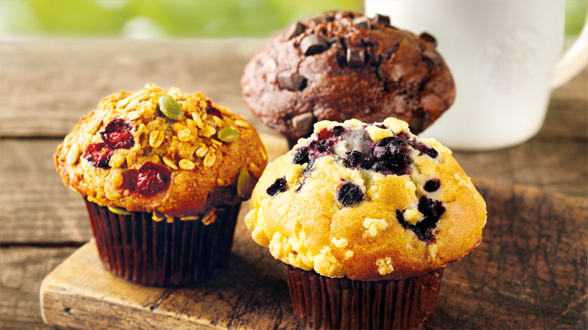
\includegraphics[width=.7\textwidth]{img/muffins.jpg} \\
     ``Wie viele Muffins von welcher Sorte?''
     \end{center}
     \end{minipage} 
       & 
     \begin{minipage}[t]{.5\textwidth}     
     \begin{center}
     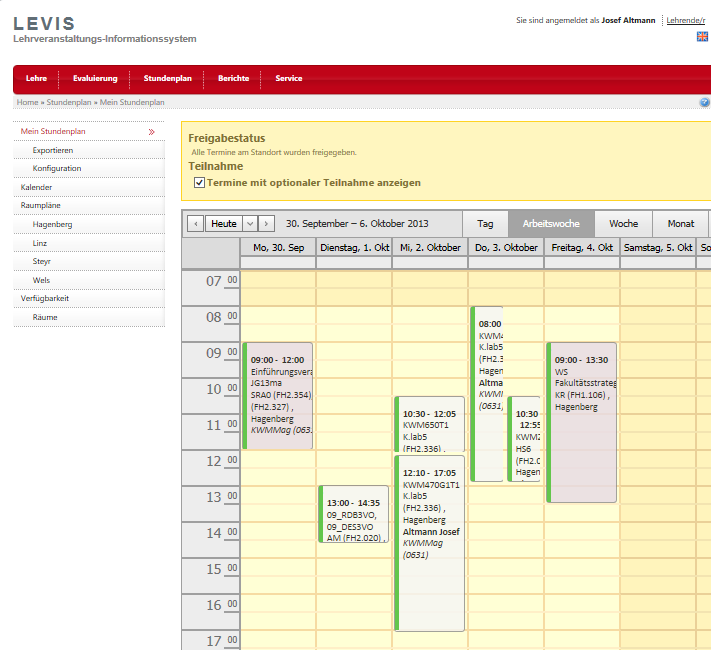
\includegraphics[width=.45\textwidth]{img/levis.png} \\
     ``Wann findet welche Vorlesung statt?''     
       \end{center}
     \end{minipage}  \\
     \begin{minipage}[t]{.45\textwidth}     
     \begin{center}
     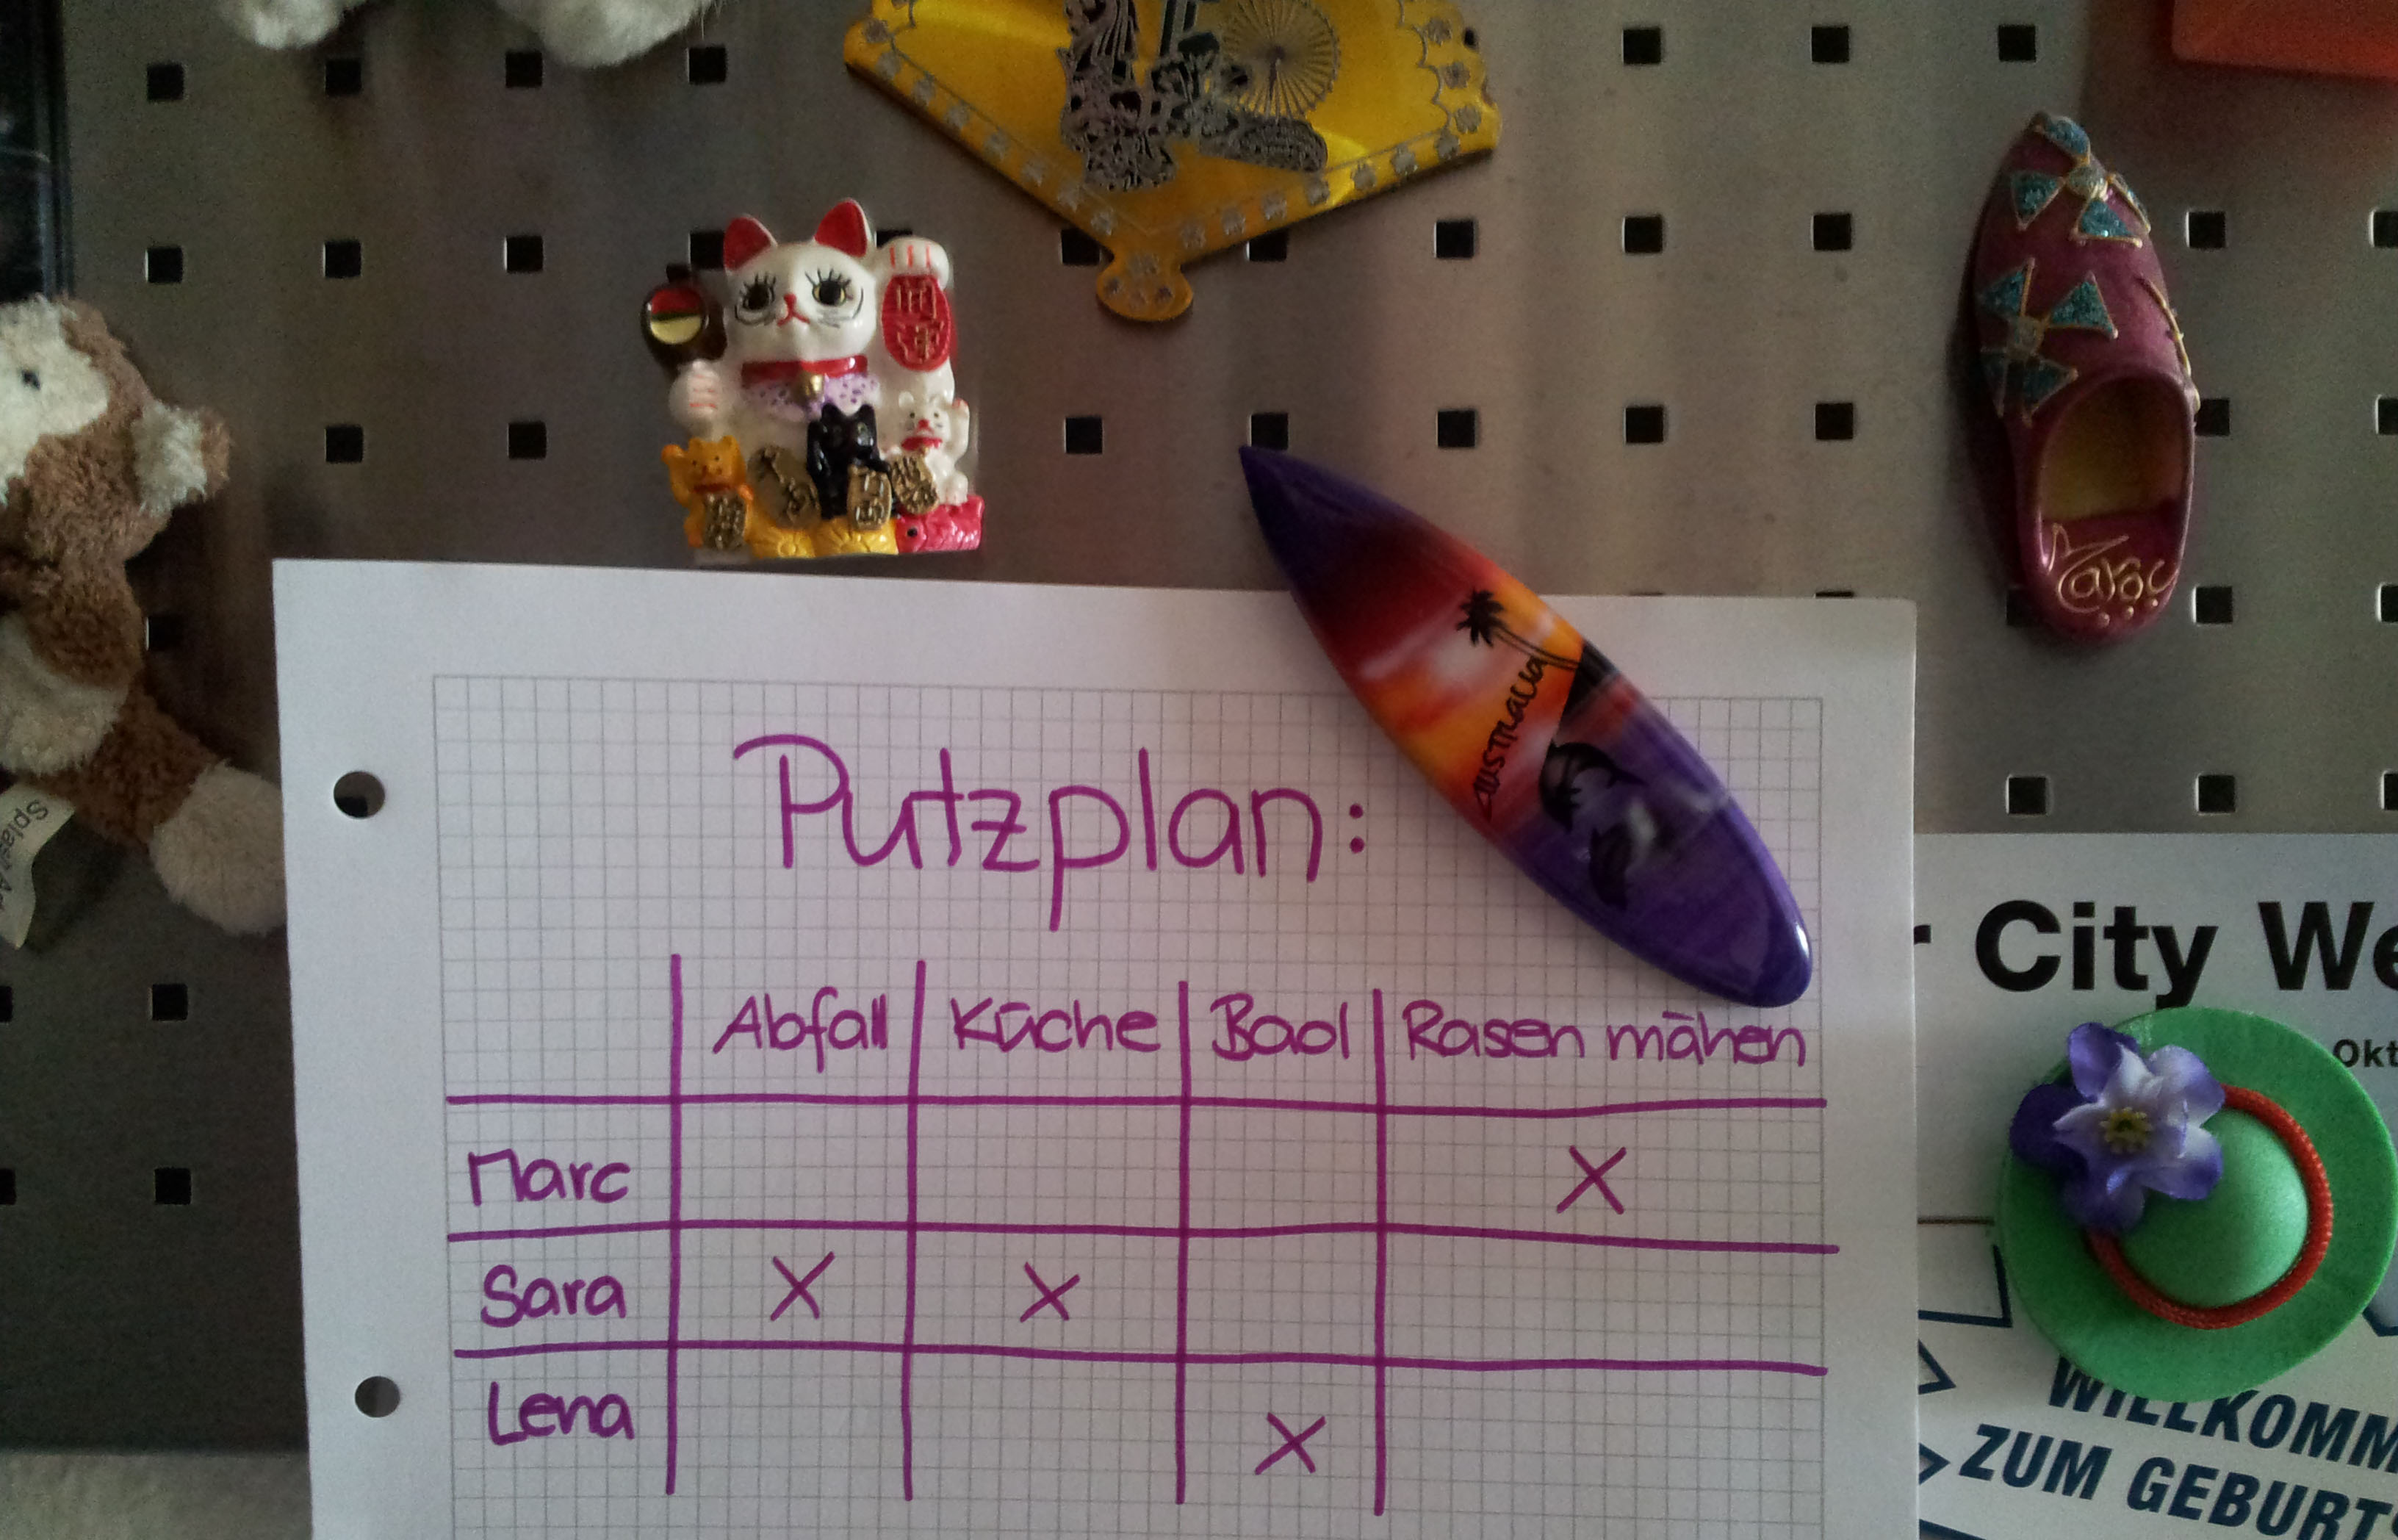
\includegraphics[width=.7\textwidth]{img/putzplan.jpg} \\
     ``Wer macht wann welche Aufgaben?''
       \end{center}
     \end{minipage}  & 
     
     \begin{minipage}[t]{.45\textwidth}
     \begin{center}
           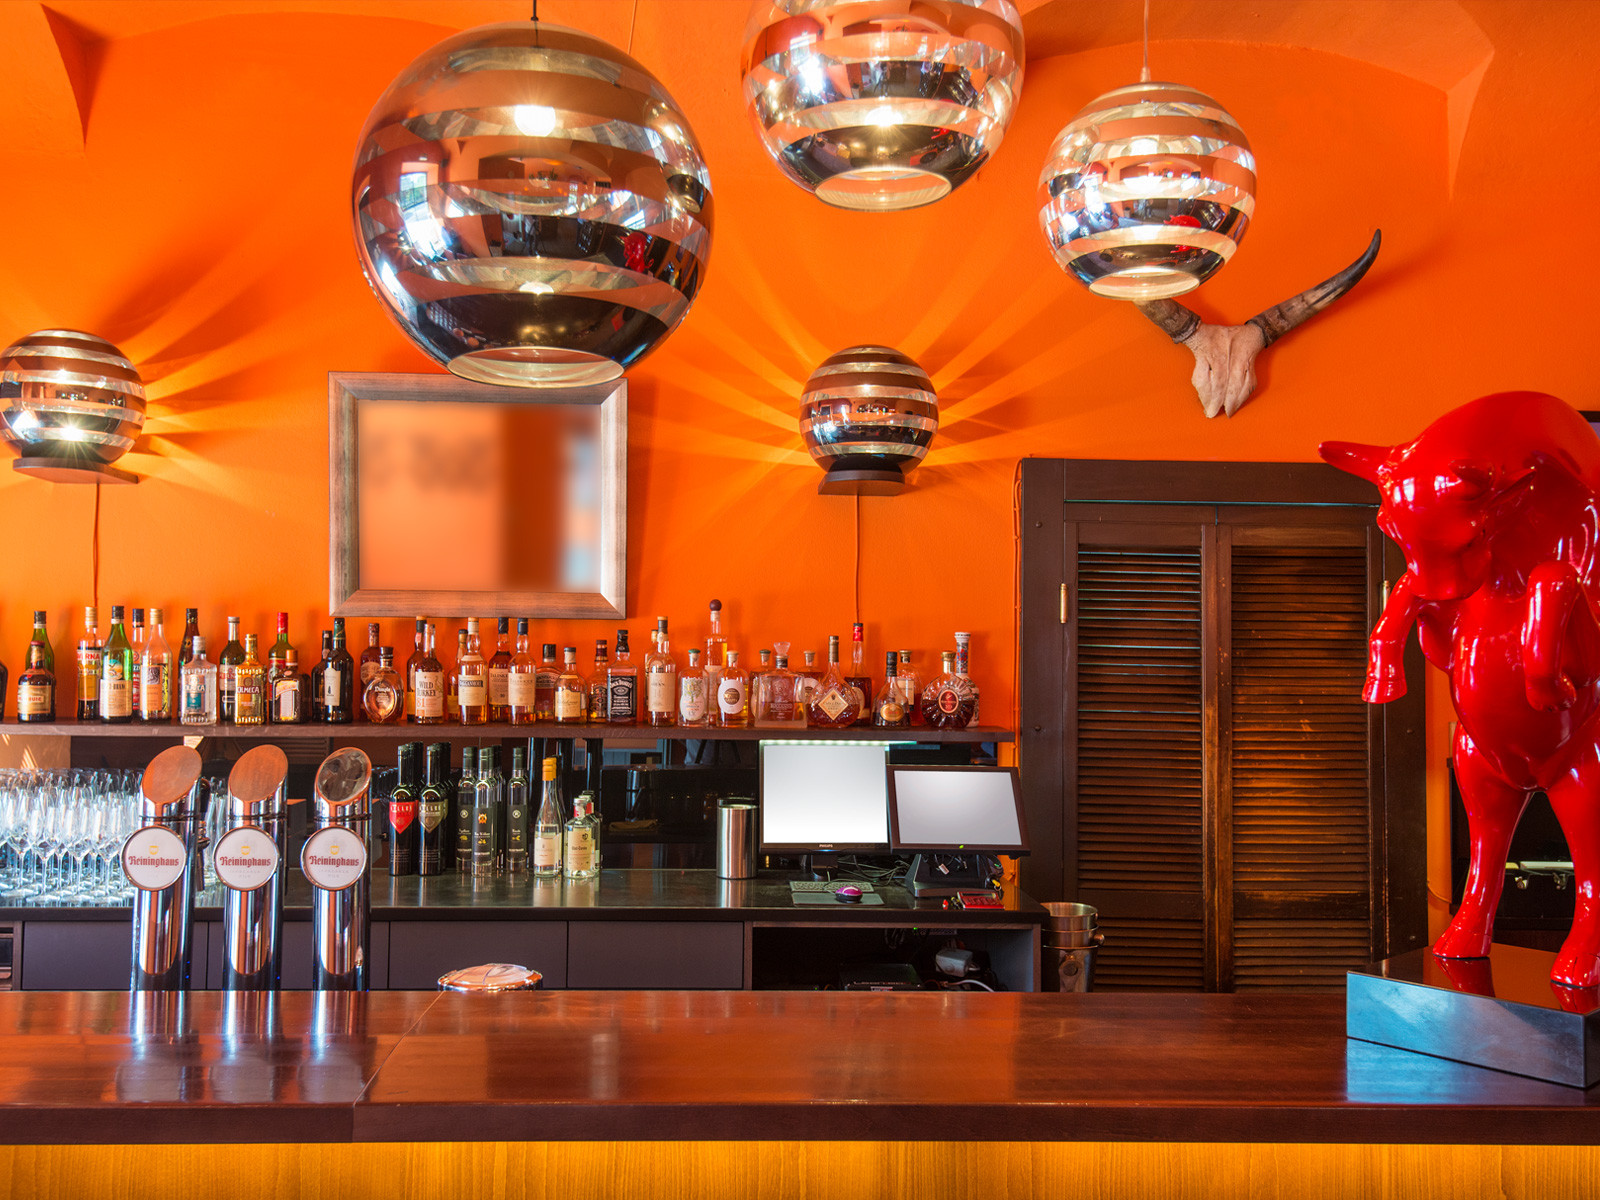
\includegraphics[width=.7\textwidth]{img/resti.jpg} \\
           ``Was machen wir am Wochenende?'' 
       \end{center}
     \end{minipage}
\\};
     
%  \path[-stealth]
%    (m-1-1) edge node [left] {$\mathcal{B}_X$} (m-2-1)
%            edge [double] node [below] {$\mathcal{B}_t$} (m-1-2)
%    (m-2-1.east|-m-2-2) edge node [below] {$\mathcal{B}_T$}
%            node [above] {$\exists$} (m-2-2)
%    (m-1-2) edge node [right] {$\mathcal{B}_T$} (m-2-2)
%            edge [dashed,-] (m-2-1);
\end{tikzpicture}

\end{center}
\end{frame}

\begin{frame}{Was haben diese Probleme gemeinsam?}
\hFirst{Entscheidungen} \onslide<2->{\emph{(Variablen)}}
\begin{itemize}
\item Die Anzahl Schokomuffins oder Bananenmuffins
\item Die Vorlesungen im Studienplan
\item Die Freitags- und Samstagsaktivität
\end{itemize}
\pause

\vspace*{2ex}

\hFirst{Möglichkeiten} \onslide<3->{\emph{(Domänen)}}
\begin{itemize}
\item Schokomuffins: $\{0, \ldots, 20\}$
\item Vorlesung ``Algorithmen 1'': $\{\mathrm{HS1}, \mathrm{HS2}, \mathrm{HS3}, \ldots \}$
\end{itemize}

\pause

\vspace*{2ex}

\hFirst{Abhängigkeiten} \onslide<4->{\emph{(Constraints)}}
\begin{itemize}
\item Das benötigte Mehl für $x$ Schoko- und $y$ Bananenmuffins darf 250g nicht übersteigen.
\item In einem Raum kann gleichzeitig nur eine Veranstaltung stattfinden.
\item Es darf nur 1 Schnitzlnight pro Wochenende geben.
\end{itemize} \pause 
\end{frame}

\begin{frame}{Was haben diese Probleme gemeinsam?}
\hFirst{Präferenzen} \onslide<2->{\emph{(Soft Constraints)}}
\begin{itemize}
\item Am Freitag, 08:00 \emph{sollte} keine Algorithmenübung stattfinden
\item Bernd möchte ins Steakhouse, Ada zur Burgerei $\rightarrow$ Adas Präferenz ist \emph{wichtiger}
\item Ich möchte weder putzen noch staubsaugen; Putzen ist aber \emph{schlimmer}
\end{itemize}
\pause

\vspace*{2ex}
und/oder
\vspace*{2ex}

\hFirst{Ziele} \onslide<3->{\emph{(Zielfunktionen)}}
\begin{itemize}
\item Maximiere den Ertrag durch Schoko/Bananenmix
\item Maximiere die Anzahl der vorlesungsfreien Tage
\end{itemize}

\vspace*{2ex}
\hfill ein \alert{Constraint-Satisfaction-(Optimization)-Problem} (CSP/COP)
\end{frame}

\begin{frame}{Autonome Systeme I: Adaptive Produktion}

\begin{center}
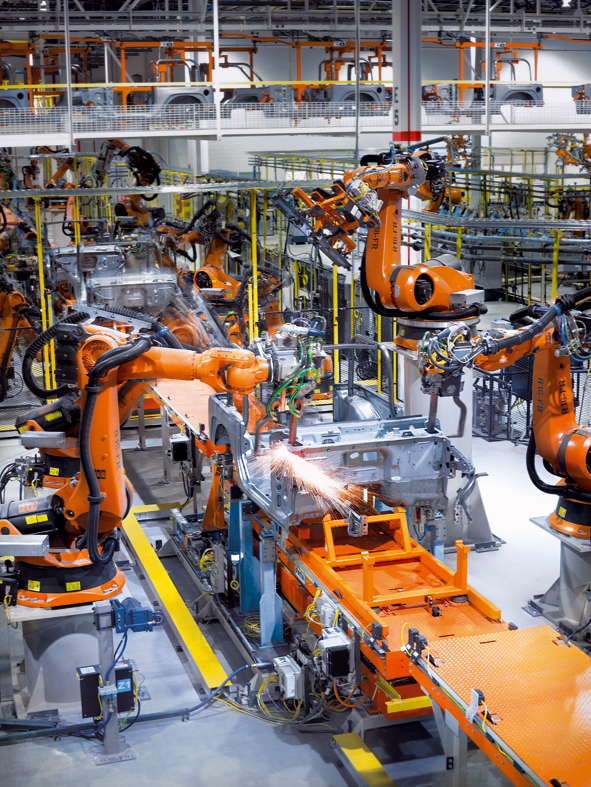
\includegraphics[width=.45\textwidth]{img/automobilindustrie.jpg}
\end{center}
\end{frame}


\begin{frame}{Autonome Systeme I: Adaptive Produktion}

\textbf{Ziel}: Weise Robotern Aufgaben so zu, dass sich ein korrekter Ressourcenfluss ergibt
\begin{center}
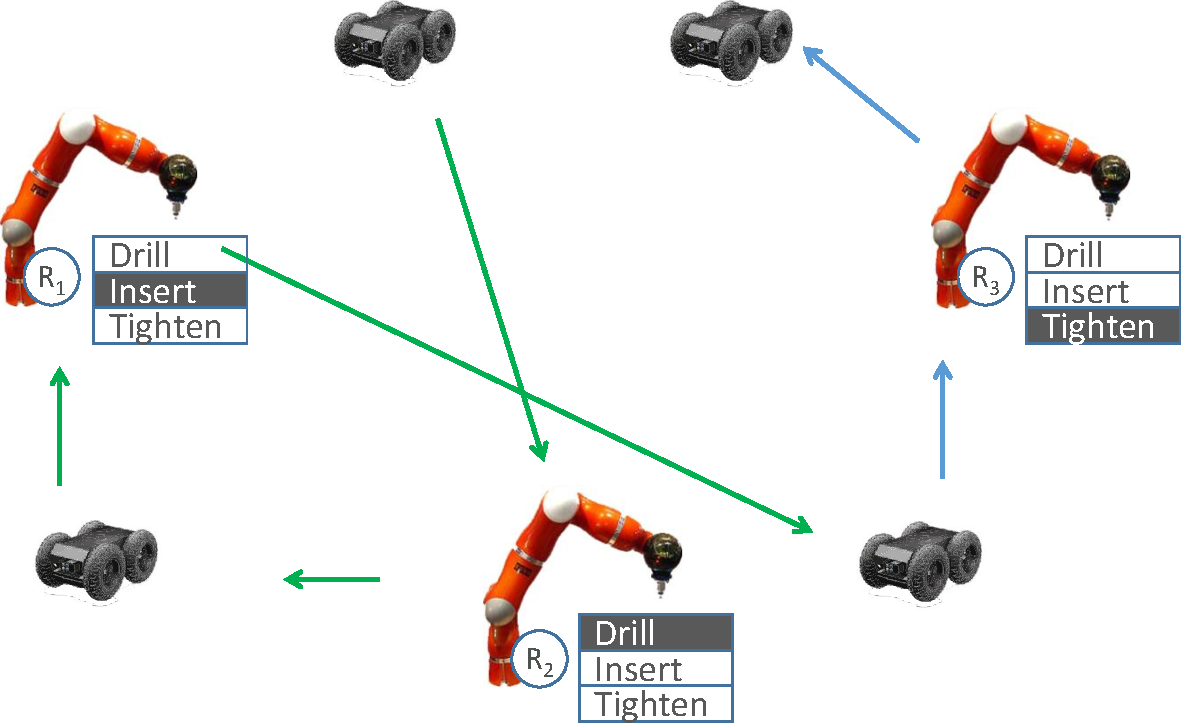
\includegraphics[width=.7\textwidth]{img/produktionszelle.pdf}
\end{center}
\end{frame}

\begin{frame}{Autonome Systeme II: Energiemanagement}
\begin{center}
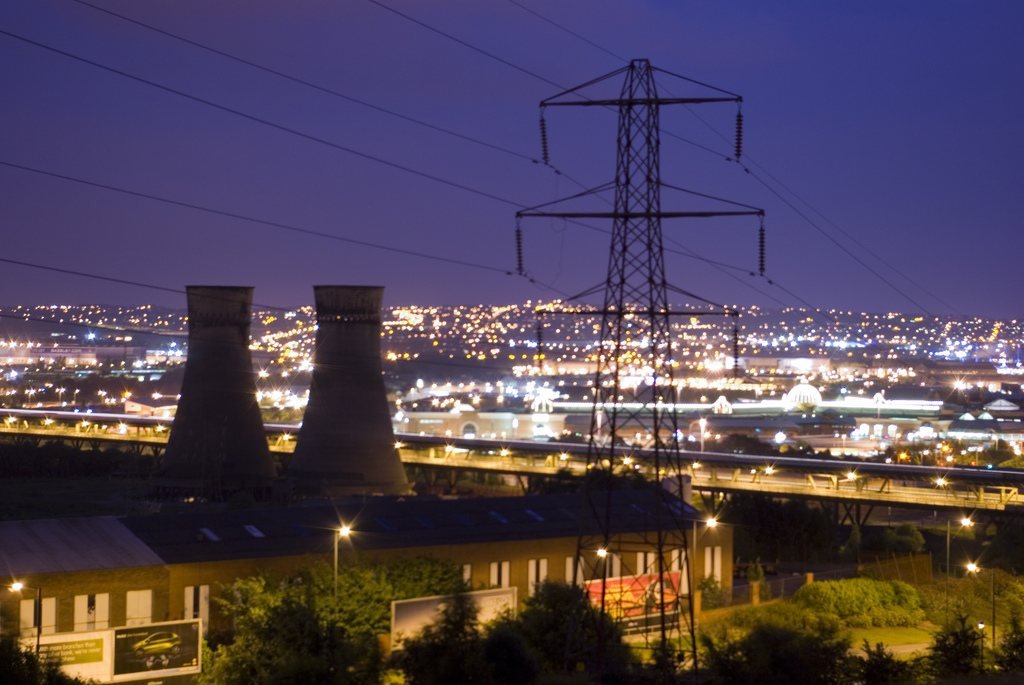
\includegraphics[width=.7\textwidth]{img/power_plants.jpg}
\end{center}
\end{frame}

\begin{frame}[fragile]{Autonome Systeme II: Energiemanagement}
\textbf{Ziel}: Plane Kraftwerke so ein, dass sie die \alert{Last} gemeinsam erfüllen
\tikzset{
    trajectory/.style={issegrey},
    emph/.style={isseorange},
    trajectorynode/.style={issegrey},
    demand/.style={MidnightBlue, thick},
    firstTraj/.style={ForestGreen},
    secTraj/.style={BrickRed}
} 
\begin{figure}
\begin{tikzpicture}[scale=1.0]
    % Draw axes
    \draw [<->,thick] (0,5) node (yaxis) [above] {$P(t)$}
        |- (8.5,0) node (xaxis) [right] {$t$};
        
    \node[overlay,text width=1.9cm, text centered, anchor=south, right] at (7.7,4.5)
    { \small 
    \begin{itemize} 
    \item[] { \color{MidnightBlue} \onslide<2->{\textbf{Demand}} } 
    \item[] { \color{ForestGreen} \onslide<3->{Plant $a$} } 
    \item[] { \color{BrickRed} \onslide<4->{Plant $b$} }  
    \item[] { \color{isseorange} \onslide<5->{\textbf{Supply}} }    
    \end{itemize}
    };        
       
	
%	\node[text width = 1.5cm ,text centered, anchor=west, right] at (2.5, 1)
%	{
%		$\mathbf{+}$
%	};
	
    %\node[text width=2.5cm, text centered, anchor=west, right] at (4,-.5)
    %{
    %		Kraftwerk $\mathsf{b}$
	%}; 
	
	%\node[text width = 1.5cm ,text centered, anchor=west, right] at (6.5, 1)
	%{
	%	$\mathbf{=}$
%	};
	%\node[text width=2.5cm, text centered, anchor=west, right] at (8,-.5)
    %{
    %		Demand
	%};      
    
     % draw second trajectory first graph 
     \onslide<2->{
    \draw[trajectory,demand] (0,3.9) coordinate (d20) -- (1,4.6) coordinate (d21);
    \draw[trajectory,demand] (d21) -- (2,4.4) coordinate (d22);
    \draw[trajectory,demand] (d22) -- (3,4.7) coordinate (d23);
    \draw[trajectory,demand] (d23) -- (4,3.5) coordinate (d24);
    \draw[trajectory,demand] (d24) -- (5,3.5) coordinate (d25);
    \draw[trajectory,demand] (d25) -- (6,3.5) coordinate (d26);
    \draw[trajectory,demand] (d26) -- (7,4.0) coordinate (d27);
    \draw[trajectory,demand] (d27) -- (8,4.5) coordinate (d28);
    
    % now for the circles
    \fill[trajectorynode,demand] (d21) circle (1pt);
    \fill[trajectorynode,demand] (d22) circle (1pt);
    \fill[trajectorynode,demand] (d23) circle (1pt);
    \fill[trajectorynode,demand] (d24) circle (1pt);    
    \fill[trajectorynode,demand] (d25) circle (1pt);
    \fill[trajectorynode,demand] (d26) circle (1pt);
    \fill[trajectorynode,demand] (d27) circle (1pt);
    \fill[trajectorynode,demand] (d28) circle (1pt);
    }
        
    \onslide<3->{
    % now for the first plant   
    \draw[trajectory,firstTraj] (0,1.9) coordinate (p10) -- (1,2.0) coordinate (p11);
    \draw[trajectory,firstTraj] (p11) -- (2,2.4) coordinate (p12);
    \draw[trajectory,firstTraj] (p12) -- (3,2.4) coordinate (p13);
    \draw[trajectory,firstTraj] (p13) -- (4,2.2) coordinate (p14);
    \draw[trajectory,firstTraj] (p14) -- (5,2.4) coordinate (p15);
    \draw[trajectory,firstTraj] (p15) -- (6,2.4) coordinate (p16);
    \draw[trajectory,firstTraj] (p16) -- (7,2.4) coordinate (p17);                   
    \draw[trajectory,firstTraj] (p17) -- (8,2.6) coordinate (p18);
    
    	\onslide<6>{
       \draw[trajectory,firstTraj,very thick] (p11) -- (p12);	
       \node[overlay,align=left,rectangle callout,%
             callout absolute pointer=(p11.west),xshift=-.5cm,yshift=-1.5cm,fill=isseorange!50] at (p12) {
            \scriptsize \textbf{Must} ramp up \\ \scriptsize due to inertia};
       
	}    
    
 	\onslide<8>{
       \draw[trajectory,firstTraj,very thick] (p15) -- (p16);	
       \draw[trajectory,firstTraj,very thick] (p16) -- (p17);
       
          \node[overlay,align=left,rectangle callout,%
             callout absolute pointer=(p16.north),xshift=-.5cm,yshift=0.55cm,fill=isseorange!50] at (p15) {
           \scriptsize  Wait 2 steps for \\ \scriptsize further ramp-up};
	} 
	
    % now for the circles of the first graph
    \fill[trajectorynode,firstTraj] (p11) circle (1pt);
    \fill[trajectorynode,firstTraj] (p12) circle (1pt);
    \fill[trajectorynode,firstTraj] (p13) circle (1pt);
    \fill[trajectorynode,firstTraj] (p14) circle (1pt);    
    \fill[trajectorynode,firstTraj] (p15) circle (1pt);
    \fill[trajectorynode,firstTraj] (p16) circle (1pt);
    \fill[trajectorynode,firstTraj] (p17) circle (1pt);
    \fill[trajectorynode,firstTraj] (p18) circle (1pt);        
    }
    
    \onslide<4->{
    % now for the second plant   
    \draw[trajectory,secTraj] (0,2.0) coordinate (p20) -- (1,2.6) coordinate (p21);
    \draw[trajectory,secTraj] (p21) -- (2,2.0) coordinate (p22);
    \draw[trajectory,secTraj] (p22) -- (3,2.2) coordinate (p23);
    \draw[trajectory,secTraj] (p23) -- (4,1.5) coordinate (p24);
    \draw[trajectory,secTraj] (p24) -- (5,1.4) coordinate (p25);
    \draw[trajectory,secTraj] (p25) -- (6,1.2) coordinate (p26);
    \draw[trajectory,secTraj] (p26) -- (7,1.6) coordinate (p27);                   
    \draw[trajectory,secTraj] (p27) -- (8,1.9) coordinate (p28);
	\onslide<6>{
       \draw[trajectory,secTraj,very thick] (p21) -- (p22);	
       \node[overlay,align=left,rectangle callout,%
             callout absolute pointer=(p21.north),xshift=+1cm,yshift=.5cm,fill=isseorange!50] at (p21) {
            \scriptsize Has to compensate};
	}    
	
	\onslide<7>{
       \draw[trajectory,secTraj,very thick] (p23) -- (p24);	
       \node[overlay,align=left,rectangle callout,%
             callout absolute pointer=(p24.south),xshift=+1cm,yshift=-.8cm,fill=isseorange!50] at (p24) {
             \scriptsize Cannot ramp down further};
	}    
    
     % now for the circles of the second graph
    \fill[trajectorynode,secTraj] (p21) circle (1pt);
    \fill[trajectorynode,secTraj] (p22) circle (1pt);
    \fill[trajectorynode,secTraj] (p23) circle (1pt);
    \fill[trajectorynode,secTraj] (p24) circle (1pt);    
    \fill[trajectorynode,secTraj] (p25) circle (1pt);
    \fill[trajectorynode,secTraj] (p26) circle (1pt);
    \fill[trajectorynode,secTraj] (p27) circle (1pt);
    \fill[trajectorynode,secTraj] (p28) circle (1pt);
    }
    
    \onslide<5->{
    % draw joint production first graph 
    \draw[trajectory,emph] (0,3.9) coordinate (s20) -- (1,4.6) coordinate (s21);
    \draw[trajectory,emph] (s21) -- (2,4.4) coordinate (s22);
    \draw[trajectory,emph] (s22) -- (3,4.6) coordinate (s23);
    \draw[trajectory,emph] (s23) -- (4,3.7) coordinate (s24);
    \draw[trajectory,emph] (s24) -- (5,3.8) coordinate (s25);
    \draw[trajectory,emph] (s25) -- (6,3.6) coordinate (s26);
    \draw[trajectory,emph] (s26) -- (7,4.0) coordinate (s27);
    \draw[trajectory,emph] (s27) -- (8,4.5) coordinate (s28);
    
	% now for the circles of the sum
    \fill[trajectorynode,emph] (s21) circle (1pt);
    \fill[trajectorynode,emph] (s22) circle (1pt);
    \fill[trajectorynode,emph] (s23) circle (1pt);
    \fill[trajectorynode,emph] (s24) circle (1pt);    
    \fill[trajectorynode,emph] (s25) circle (1pt);
    \fill[trajectorynode,emph] (s26) circle (1pt);
    \fill[trajectorynode,emph] (s27) circle (1pt);
    \fill[trajectorynode,emph] (s28) circle (1pt);
    }
    
	\node[text centered, anchor=north] at (1,0) { 1 }; \draw[thick] (1,0.05) -- (1,-.05);
	\node[text centered, anchor=north] at (2,0) { 2 }; \draw[thick] (2,0.05) -- (2,-.05);
	\node[text centered, anchor=north] at (3,0) { 3 }; \draw[thick] (3,0.05) -- (3,-.05);	
	\node[text centered, anchor=north] at (4,0) { 4 }; \draw[thick] (4,0.05) -- (4,-.05);
	\node[text centered, anchor=north] at (5,0) { 5 }; \draw[thick] (5,0.05) -- (5,-.05);
	\node[text centered, anchor=north] at (6,0) { 6 }; \draw[thick] (6,0.05) -- (6,-.05);
	\node[text centered, anchor=north] at (7,0) { 7 }; \draw[thick] (7,0.05) -- (7,-.05);	
	\node[text centered, anchor=north] at (8,0) { 8 }; \draw[thick] (8,0.05) -- (8,-.05);
	    

\end{tikzpicture}
\end{figure}  
\end{frame}

\begin{frame}{Ein klassisches CSP}
\begin{center}
\chessboard[clearboard,setpieces={Qf8, Qc7, Qe6, Qh5, Qa4, Qd3, Qb2, Qg1}]
\end{center}
\end{frame}

\begin{frame}{Klassischer Ansatz}
Entwickle eigenen Algorithmus \emph{from scratch}:
\begin{center}
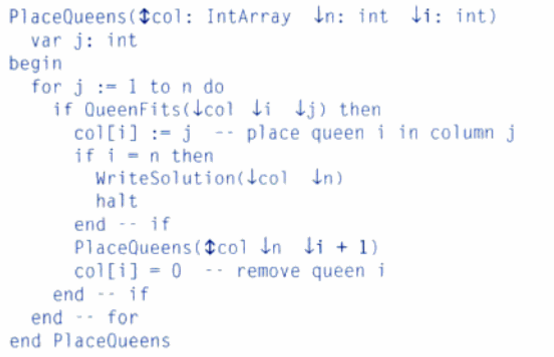
\includegraphics[width=.7\textwidth]{img/algo.png}
\end{center}
\hfill \emph{(Pomberger, Dobler, 2008)}
\end{frame}

\begin{frame}[fragile]{Modellieren statt Programmieren!}
\alert{Alternative}: Schreibe \emph{ein} Modell -- teste \emph{viele} Algorithmen!

\vspace*{1ex}

\lstinputlisting{models/soft-queens-0.mzn}
\begin{tikzpicture}
\matrix (m) [matrix of nodes,row sep=0.2em,column sep=0em,minimum width=1em]
  {
  2 & 3 & 4 & 5 & \qquad & \qquad & \qquad & 0 & -1 & -2 & -3 \\
  3 & 4 & 5 & 6 & \qquad & \qquad & \qquad & 1 & 0 & -1 & -2 \\
  4 & 5 & 6 & 7 & \qquad & \qquad & \qquad & 2 & 1 & 0 & -1 \\
  5 & 6 & 7 & 8 & \qquad & \qquad & \qquad & 3 & 2 & 1 & 0 \\  
  };
     
%  \path[-stealth]
%    (m-1-1) edge node [left] {$\mathcal{B}_X$} (m-2-1)
%            edge [double] node [below] {$\mathcal{B}_t$} (m-1-2)
%    (m-2-1.east|-m-2-2) edge node [below] {$\mathcal{B}_T$}
%            node [above] {$\exists$} (m-2-2)
%    (m-1-2) edge node [right] {$\mathcal{B}_T$} (m-2-2)
%            edge [dashed,-] (m-2-1);
\end{tikzpicture}

\small
\begin{verbatim}
queens = array1d(1..8 ,[4, 6, 1, 5, 2, 8, 3, 7]);
----------
\end{verbatim}
\copyright~Hakan Kjellerstrand, \url{http://www.hakank.org/minizinc}
\end{frame}

\begin{frame}
    \frametitle{Soft Constraint Programming in MiniBrass}
 \alert{Constraint Programming}
    \begin{itemize}
    \item Deklarative Programmierung (ähnlich SQL, Prolog)
    \item Trennung von \textbf{Modell} und \emph{Algorithmus}
    \item Geeignet für kombinatorische Probleme unter harten Bedingungen (Physik!)
    \item Modellierungssprache \hFirst{MiniZinc}
    \end{itemize}

    \vspace*{3ex}
    
\alert{Soft Constraint Programming}
    \begin{itemize} 
    \item Modellierung von \textbf{Nutzerpräferenzen}
    \item Finde Lösungen, die \emph{so gut wie möglich} sind
    \item Was bedeutet ``gut``?
    \item Modellierungssprache \hFirst{MiniBrass}
     \end{itemize}
\end{frame}

\begin{frame}{Künstliche Intelligenz: Einteilung}
\begin{columns}[onlytextwidth,T]
    
    \begin{column}{.5\textwidth}
          
    \hSecond{Data-driven AI}
    \begin{center}
    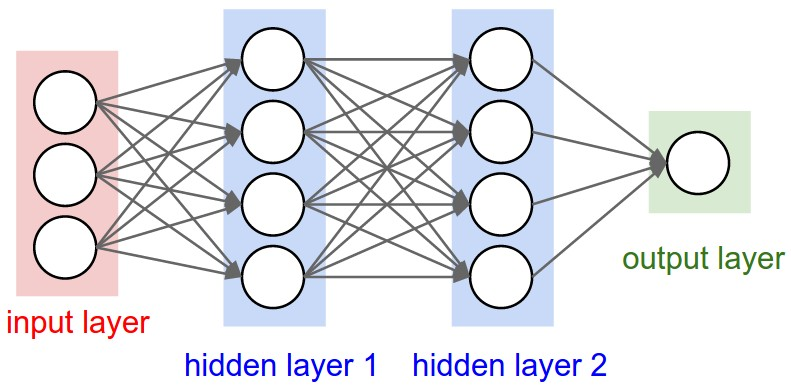
\includegraphics[width=.8\textwidth]{img/neuralnet.jpg}
    \end{center}

    \vspace*{4ex}
    
    \begin{itemize}
    \item Machine Learning
    \item Signal Processing
    \item Computer Vision
    \end{itemize}

    \end{column}
    
    \begin{column}{.5\textwidth}
    \hFirst{Decision-driven AI}
    \begin{center}
    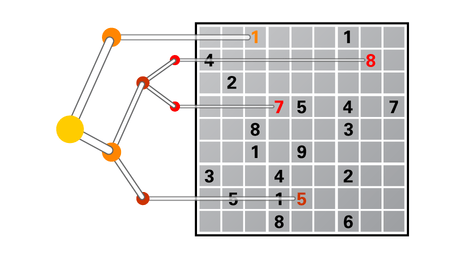
\includegraphics[width=.9\textwidth]{img/discreteopt.png}
    \end{center}
    \begin{itemize}
    \item Constraint Programming
    \item Combinatorial Optimization
    \item Heuristic Optimization
    \item Planning / Scheduling
    \end{itemize}
    
    \end{column}
  \end{columns}
\end{frame}

\begin{frame}{Warum modellieren?}
\begin{enumerate}
\item Einmal (formal) modelliert -- vielseitig gelöst
\begin{itemize}
\item Constraint-Solving
\item SAT
\item MIP 
\item Heuristiken
\end{itemize}
\vspace*{1ex}
\item Effiziente, (normalerweise) gut getestete Algorithmen in Lösern verbaut
\begin{itemize}
\item Gleiche Algorithmen für viele Probleme
\item Spezialalgorithmen für wiederkehrende Teilprobleme (\texttt{alldifferent})
\end{itemize}
\vspace*{1ex}
\item Prototyping
\begin{itemize}
\item Problemspezifikation wird klarer
\item Spezialalgorithmus für konkretes Problem kann nachentwickelt werden
\end{itemize}

\end{enumerate}
\end{frame}

\begin{frame}[fragile]{Verwandte Technik}
\begin{lstlisting}[language=sql]
SELECT firstname, lastname
FROM employees 
WHERE age < 30
\end{lstlisting}
\vspace*{1ex}
statt 
\vspace*{1ex}
\begin{lstlisting}[language=java]
Collection<Person> youngs = new ArrayList<>();
for(Person p : allEmployees) {
  if(p.getAge() < 30)
    youngs.add(p);
}
\end{lstlisting}

\begin{parchment}[Motivation]
\centering 
\alert{Constraint-Modellierung für Optimierungsprobleme $\approx$ SQL für Datenzugriff} 
\end{parchment}

\end{frame}

\begin{frame}{NP-Vollständigkeit}
\begin{theorem}
Das zu einem CSP gehörende Entscheidungsproblem ist NP-vollständig.
\end{theorem}

\begin{center}
\begin{figure}
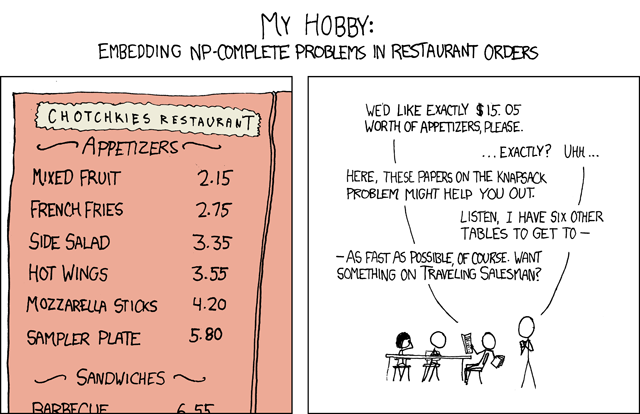
\includegraphics[width=.8\textwidth]{img/np_complete.png}
\caption{\url{https://xkcd.com/287/} }
\end{figure}
\end{center}
\end{frame}

\begin{frame}{Warum MiniZinc?}
\begin{parchment}[Rationale]
\centering 
\alert{Eine Sprache -- viele Solver} 
\end{parchment}
\begin{textblock*}{2.cm}[1,1](\textwidth-.5cm,\textheight-1.03cm)


\includegraphics[width=\textwidth]{img/MiniZn_logo.jpg} 

\end{textblock*}
Unterstützte Solver
\begin{itemize}
\item Gecode (CP)
\item JaCoP (CP)
\item Google Optimization Tools (CP)
\item Choco (CP)
\item G12 (CP/LP/MIP)
\end{itemize}

\end{frame}


\begin{frame}[fragile]{Ein erstes Modell}
\begin{lstlisting}
var 0..2: x;
var 0..2: y; 

constraint x < y;

solve maximize x + y;
\end{lstlisting}

\vspace*{2ex}

\url{http://www.minizinc.org}

\vspace*{2ex}

\small
\begin{verbatim}
x = 1;
y = 2;
----------
==========
\end{verbatim}

\end{frame}

\begin{frame}[fragile]{Etwas interessanter \ldots}
\small
\lstinputlisting{models/cakes.mzn}
\end{frame}

\begin{frame}{Task-Zuweisung in Practice}
\begin{itemize}
\item Taskzuweisungsproblem (\emph{task allocation problem})

\begin{itemize}
\item [-] $n$ Roboter
\item [-] $m$ Tasks
\item [-] Gebe jedem Roboter einen \emph{unterschiedlichen} Task, und maximiere den Gewinn 
\end{itemize}
\item Beispielproblem:
\begin{itemize}
\item[-] $n = 4$, $m = 5$
\end{itemize}
\end{itemize}
\centering
\begin{tabular}{|c|c|c|c|c|c|}
\hline 
 & t1 & t2 & t3 & t4 & t5 \\ 
\hline 
r1 & 7 & 1 & 3 & 4 & 6 \\ 
\hline 
r2 & 8 & 2 & 5 & 1 & 4 \\ 
\hline 
r3 & 4 & 3 & 7 & 2 & 5 \\ 
\hline 
r4 & 3 & 1 & 6 & 3 & 6 \\ 
\hline 
\end{tabular} 
\end{frame}


\begin{frame}[fragile]{Task-Zuweisung: Modell}
\begin{lstlisting}
% problem data 
int: n; set of int: ROBOTS = 1..n;
int: m; set of int: TASKS = 1..m;
array[ROBOTS,TASKS] of int: profit;

% decisions
array[ROBOTS] of var TASKS: allocation;

% goal
solve maximize sum(r in ROBOTS) (profit[r, allocation[r]] );

% have robots work on different tasks
constraint alldifferent(allocation);
\end{lstlisting}
\end{frame}

\begin{frame}{Wie funktioniert's?}
Im Wesentlichen \ldots 
\begin{center}
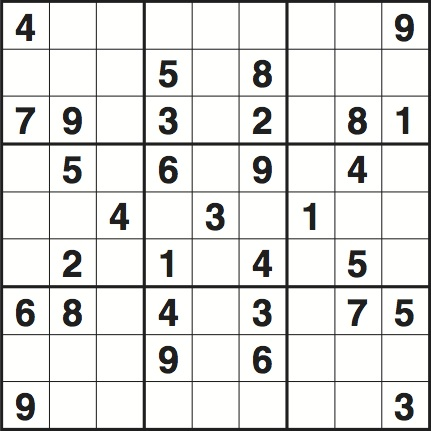
\includegraphics[width=.4\textwidth]{img/sudoku.jpg}
\end{center}
\begin{enumerate}
\item Streiche alle Kandidaten raus \onslide<2->{\emph{(Constraint Propagation)}}
\item Fülle alle Felder aus, bei denen nur noch 1 Zahl in Frage kommt
\item Wenn du nicht mehr weiterkommst $\rightarrow$ probiere aus \onslide<3->{\emph{(Backtracking Search)}}
\end{enumerate}
\end{frame}

\begin{frame}{Constraint-Propagation: Beispiel}
\begin{center}
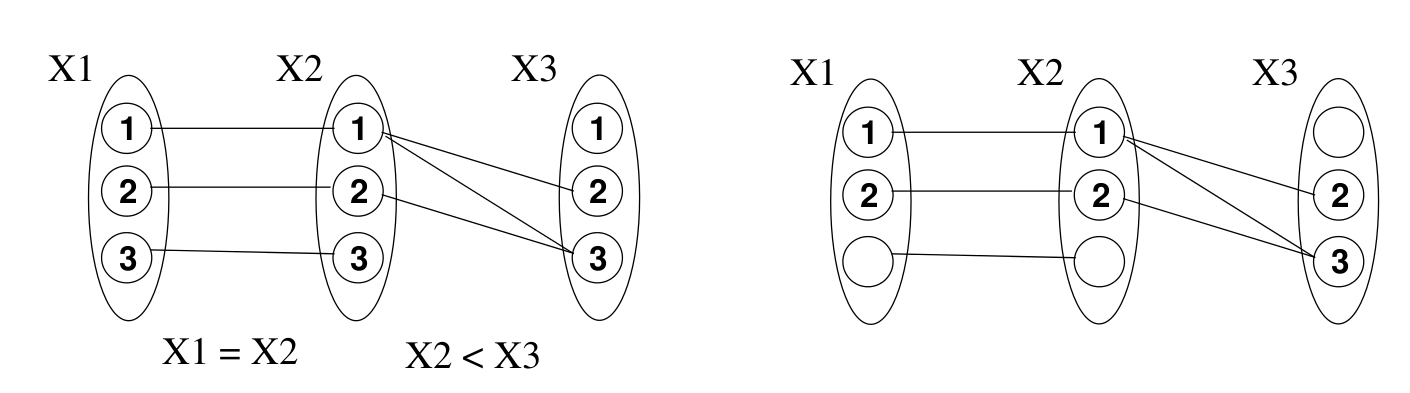
\includegraphics[width=\textwidth]{img/constprop.png}
\end{center}
Entferne Werte, die zu keiner Lösung führen können. 
\end{frame}


\graphicspath{{img/}}
\begin{frame}{Suche am Beispiel Map Coloring}
\begin{center}
\def\svgwidth{.55\columnwidth}
\input{img/australia-large-exp.pdf_tex}
\end{center}

$X = \{ \mathsf{WA}, \mathsf{NT}, \ldots \mathsf{V} \}$, $D_x = \{\mathsf{r}, \mathsf{g}, \mathsf{b} \}$, $C = \{
\mathsf{WA} \neq \mathsf{NT}, \mathsf{NT} \neq \mathsf{SA}, \ldots  \}$


\end{frame}

\begin{frame}{Systematische Suche I}

\begin{center}
\begin{tikzpicture}[auto,
                    ->,>=stealth',shorten >=1pt,thick,
                    node distance=2.7cm,inner sep=0pt,
                    constraint/.style={circle,fill=black!15,draw,font=\sffamily\small}]
\node (1) at (0, 0)                   {
\def\svgwidth{.15\columnwidth}
\input{img/australia.pdf_tex}
};

\node[below of=1] (3) {
\def\svgwidth{.15\columnwidth}
\input{img/wa-red.pdf_tex}
};  

\node[left of=3] (2) {
\def\svgwidth{.15\columnwidth}
\input{img/wa-blue.pdf_tex}
};  


\node[right of=3] (4) {
\def\svgwidth{.15\columnwidth}
\input{img/wa-green.pdf_tex}
};

\path[every node/.style={font=\sffamily\tiny}]
  (1) edge (2)
  (1) edge (3)
  (1) edge (4)
 ;

\node[below left of=2] (5) {
\def\svgwidth{.15\columnwidth}
\input{img/blue-red.pdf_tex}
};

\node[below right of=2] (6) {
\def\svgwidth{.15\columnwidth}
\input{img/blue-green.pdf_tex}
};
%  
\path[every node/.style={font=\sffamily\tiny}]
  (2) edge (5)
  (2) edge (6)
  ;
\end{tikzpicture}
\end{center}
\end{frame}

\begin{frame}{Systematische Suche II}

\begin{center}
\begin{tikzpicture}[auto,
                    ->,>=stealth',shorten >=1pt,thick,
                    node distance=2.7cm,inner sep=0pt,
                    constraint/.style={circle,fill=black!15,draw,font=\sffamily\small}]
\node (1) at (0, 0)                   {
\def\svgwidth{.15\columnwidth}
\input{img/blue-red.pdf_tex}
};

\node[below left of=1] (2) {
\def\svgwidth{.15\columnwidth}
\input{img/wa-red-green.pdf_tex}

{\huge
\alert{\Lightning}
}
};  

\node[below right of=1] (3) {
\def\svgwidth{.15\columnwidth}
\input{img/wa-red-blue.pdf_tex}
};  

\path[every node/.style={font=\sffamily\tiny}]
  (1) edge (2)
  (1) edge (3)
 ;

\node[below of=3] (5) {
\def\svgwidth{.15\columnwidth}
\input{img/wa-red-green-blue.pdf_tex}
};
%  
\path[every node/.style={font=\sffamily\tiny}]
  (3) edge (5)
  ;
\end{tikzpicture}
\end{center}

\end{frame}

\begin{frame}{Tricks (Heuristiken)}
Wähle Länder (Variablen) und Farben (Werte) in \alert{geschickter} Reihenfolge aus


\begin{itemize}
\item \emph{Minimum-Remaining-Values} (MRV): Wähle das Land mit der kleinsten verbleibenden Domäne 
\item \emph{Most-constrained} (MC): Wähle das Land mit den meisten angrenzenden Ländern
\item \emph{Minimum reduction} (MR): Wähle eine Farbe, die andere Länder minimal einschränkt
\end{itemize}

Dadurch frühe Sackgassenerkennung und sinnvolle Wahl, um Suchbaum zu begrenzen.
\end{frame}

\begin{frame}{Variablenordnung}
Beispiel für MRV+MC (MC bricht Unentschieden nach MRV):

\begin{tikzpicture}
  \matrix[ampersand replacement=\&]
  {
    \node (i1) {
    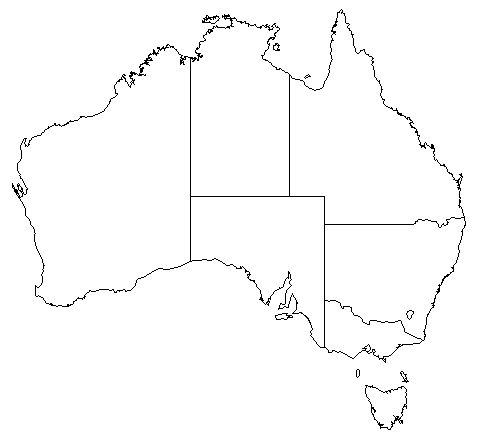
\includegraphics[width=.2\textwidth]{australia.pdf}}; \&[2mm]  
    \node(i2){
    
\includegraphics[width=.2\textwidth]{st-red.pdf}}; \&[2mm]
    \node(i3){
    
\includegraphics[width=.2\textwidth]{st-red-ql-blue.pdf}}; \&[2mm]
	\node(i4){
    
\includegraphics[width=.2\textwidth]{st-red-ql-blue-nt-green.pdf}};
    \\ 
	\node (l1) {Alle unbelegt}; \& 
	\node (l2) {SA in 5 Constraints}; \&
	\node(l3){$|D_\mathsf{QL}|$ nur 2 }; \&	
	\node(l4){$|D_\mathsf{NT}|$ nur 1 }; \&	
		
	\\
  };
  
\end{tikzpicture}
\end{frame}

\begin{frame}{Wertordnung}
Wähle die Belegung, die
die wenigsten Domäneneinschränkungen zur Folge haben.
\begin{center}
\begin{tikzpicture}[auto,
                    ->,>=stealth',shorten >=1pt,thick,
                    node distance=2.6cm,inner sep=0pt,
                    constraint/.style={circle,fill=black!15,draw,font=\sffamily\small}]
\node (1) at (0, 0)                   {
\def\svgwidth{.15\columnwidth}
\input{img/blue-red.pdf_tex}
};

\node[below left of=1] (2) {
\def\svgwidth{.15\columnwidth}
\input{img/wa-red-green.pdf_tex}

{\huge
\alert{\Lightning}
}
};  

\node[below right of=1] (3) {
\def\svgwidth{.15\columnwidth}
\input{img/wa-red-blue.pdf_tex}
};  


\node[below left of=2] (l2) {
Es bleibt \alert{kein} Wert für SA.
};

\node[below right of=3] (l3) {
Es bleibt ein Wert für SA.
};


\path[every node/.style={font=\sffamily\tiny}]
  (1) edge (2)
  (1) edge (3)
 ;
\end{tikzpicture}
\end{center}
\end{frame}

\begin{frame}[fragile]{Erstes Modell: Revisited}
\begin{lstlisting}
var 0..2: x;
var 0..2: y; 

constraint x < y;

solve
:: int_search([x,y], input_order, indomain_max, complete)
maximize x + y;\end{lstlisting}


\vspace*{2ex}

\small
\begin{verbatim}
x = 1;
y = 2;
----------
==========
\end{verbatim}

\end{frame}

\begin{frame}
\frametitle{Soft Constraint Solving}

\vspace*{1ex}

In der Praxis: \cemph{überbestimmte} Probleme

\vspace*{2ex}

$x, y, z \in \{1,2,3\}$ mit 
\bgroup\abovedisplayskip4pt\belowdisplayskip4pt
\begin{align*}
  \mathrm{c}_1 &: x + 1 = y
\\[-.4ex]
  \mathrm{c}_2 &: z = y + 2
\\[-.4ex]
  \mathrm{c}_3 &: x + y \leq 3
\end{align*}
\egroup

\begin{itemize}
  \item Nicht alle Constraints können gleichzeitig erfüllt werden
\begin{itemize} \pause
  \item e.\,g., $\mathrm{c}_2$ erzwingt $z = 3$ und $y = 1$, im Konflikt mit $\mathrm{c}_1$
\end{itemize}

  \item Wir \cemph{wählen} zwischen Zuweisungen, die $\{ \mathrm{c}_1, \mathrm{c}_3 \}$ oder $\{ \mathrm{c}_2, \mathrm{c}_3 \}$ erfüllen.
\end{itemize}

\vspace*{2ex}

Welche Zuweisungen $v \in [X \to D]$ sollen \alert{bevorzugt} werden?

\end{frame}

\begin{frame}
\frametitle{Constraint Relationships}

Ansatz~\cite{Schiendorfer13}
\begin{itemize}
  \item Definiere Relation $R$ über Constraints $C$ um anzugeben, welche Constraints wichtiger sind als andere, e.\,g.
\begin{itemize}
  \item $\mathrm{c}_1$ wichtiger als $\mathrm{c}_2$

  \item $\mathrm{c}_1$ wichtiger als $\mathrm{c}_3$
\end{itemize}
\end{itemize}
\begin{textblock*}{2.5cm}[1,1](\textwidth-1.5cm,\textheight-2.03cm)
\begin{tikzpicture}[auto,
                    ->,>=stealth',shorten >=1pt,thick,
                    node distance=.7cm,inner sep=2pt,
                    constraint/.style={circle,fill=black!15,draw,font=\sffamily\small}]
\node[constraint node] (1) at (0, 0)                   {$\mathrm{c}_1$};
\node[constraint node] (2) at ($ (1) + (-0.8, -0.8) $) {$\mathrm{c}_2$};  
\node[constraint node] (3) at ($ (1) + ( 0.8, -0.8) $) {$\mathrm{c}_3$};  
%  
\path[every node/.style={font=\sffamily\tiny}]
  (2) edge (1)
  (3) edge (1)
  ;
\end{tikzpicture}
\end{textblock*}

%\vspace*{2ex}
%\begin{small}
%A.~Schiendorfer, J.-Ph.~Steghöfer, A.~Knapp, F.~Nafz, W.~Reif (2013)
%\end{small}
\end{frame}

\begin{frame}[fragile]{MiniBrass}

\begin{center}

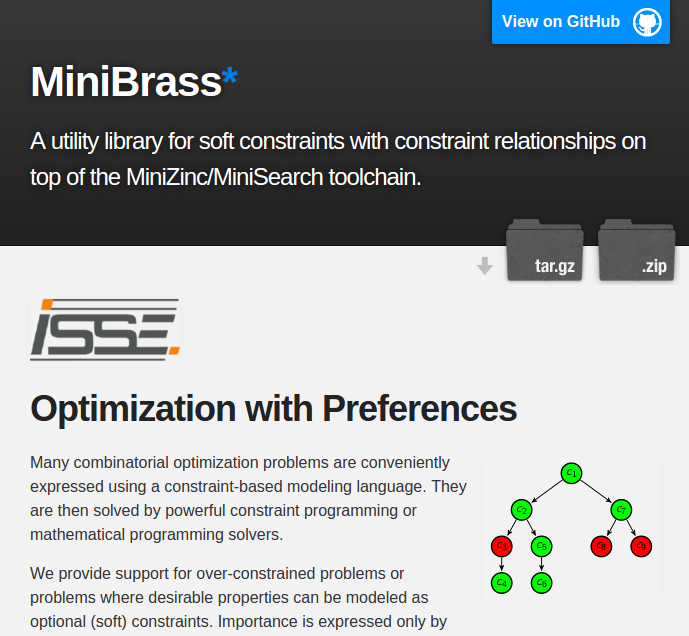
\includegraphics[width=.5\textwidth]{img/minibrass.png}

\vspace*{2ex}

\url{http://isse-augsburg.github.io/constraint-relationships/}

\end{center}

\end{frame}

\begin{frame}
\frametitle{Single-Predecessor-Dominance (SPD)}

\cemph{isWorseThan}-Relation für Mengen verletzter Constraints
%
%\bgroup\abovedisplayskip=4pt\belowdisplayskip=12pt
%\begin{gather*}
%  V \SPDrel{R} V \uplus \{ c \} 
%\\
%  V \uplus \{ c \} \SPDrel{R} V \uplus \{ c' \}
%\quad\text{if $c \rightarrow_R c'$}
%\end{gather*}
%\egroup

\begin{center}
\begin{tikzpicture}[auto,
                    ->,>=stealth',shorten >=1pt,thick,
                    node distance=1cm,inner sep=2pt,
                    constraint/.style={circle,fill=black!15,draw,font=\sffamily\small}]
\begin{scope}
\node[constraint,fill=green] (1) at (0, 0)                   {$\mathrm{c}_7$};
\node[constraint,fill=green] (2) at ($ (1) + (-1.2, -0.8) $) {$\mathrm{c}_4$};  
\node[constraint,fill=red]   (3) at ($ (2) + (0.0, -0.9) $) {$\mathrm{c}_5$};  
\node[constraint,fill=green] (4) at ($ (3) + ( 0.0, -1.0) $) {$\mathrm{c}_6$};
\node[constraint,fill=green] (7) at ($ (1) + ( 1.2, -0.8) $) {$\mathrm{c}_1$};  
\node[constraint,fill=red]   (8) at ($ (7) + (-0.6, -0.9) $) {$\mathrm{c}_2$};  
\node[constraint,fill=red]   (9) at ($ (7) + ( 0.6, -0.9) $) {$\mathrm{c}_3$};  
%  
\path[every node/.style={font=\sffamily\tiny}]
  (2) edge (1)
  (7) edge (1)
  (3) edge (2)
  (4) edge (3)
  (8) edge (7)
  (9) edge (7)
  ;
\end{scope}
%
\begin{scope}[xshift=6cm]
\node[constraint,fill=green] (1) at (0, 0)                   {$\mathrm{c}_7$};
\node[constraint,fill=red]   (2) at ($ (1) + (-1.2, -0.8) $) {$\mathrm{c}_4$};  
\node[constraint,fill=green] (3) at ($ (2) + (0.0, -0.9) $) {$\mathrm{c}_5$};  
\node[constraint,fill=green] (4) at ($ (3) + ( 0.0, -1.0) $) {$\mathrm{c}_6$};  
\node[constraint,fill=green] (7) at ($ (1) + ( 1.2, -0.8) $) {$\mathrm{c}_1$};  
\node[constraint,fill=red]   (8) at ($ (7) + (-0.6, -0.9) $) {$\mathrm{c}_2$};  
\node[constraint,fill=red]   (9) at ($ (7) + ( 0.6, -0.9) $) {$\mathrm{c}_3$};  
%  
\path[every node/.style={font=\sffamily\tiny}]
  (2) edge (1)
  (7) edge (1)
  (3) edge (2)
  (4) edge (3)
  (8) edge (7)
  (9) edge (7)
  ;
\end{scope}
%
\node (R) at (3.05, -1.4) {$\SPDrel{R}$};
\end{tikzpicture}
\end{center}
%
%\cemph{Ordnungs}relation über Zuweisungen 
%\bgroup\abovedisplayskip4pt
%\begin{equation*}
%  w \SPDord{R} v \iff \{ c \in C \mid v \not\models c \} \mathrel{({\SPDrel{R}})^{+}} \{ c \in C \mid w \not\models c \}
%\end{equation*}
%\egroup

\end{frame}


\begin{frame}
\frametitle{Transitive-Predecessors-Dominance (TPD)}

\cemph{isWorseThan}-Relation für Mengen verletzter Constraints
%
%\bgroup\abovedisplayskip=4pt\belowdisplayskip=12pt
%\begin{gather*}
%  V \TPDrel{R} V \uplus \{ c \} 
%\\
%  V \uplus \{ c_1, \ldots, c_k \} \TPDrel{R} V \uplus \{ c' \}
%\quad\text{if $\forall c \in \{ c_1, \ldots, c_k \} \,.\, c \rightarrow_{R}^{+} c'$}
%\end{gather*}
%\egroup

\begin{center}
\begin{tikzpicture}[auto,
                    ->,>=stealth',shorten >=1pt,thick,
                    node distance=1cm,inner sep=2pt,
                    constraint/.style={circle,fill=black!15,draw,font=\sffamily\small}]
\begin{scope}
\node[constraint,fill=green] (1) at (0, 0)                   {$\mathrm{c}_7$};
\node[constraint,fill=green] (2) at ($ (1) + (-1.2, -0.8) $) {$\mathrm{c}_4$};  
\node[constraint,fill=red]   (3) at ($ (2) + (0.0, -0.9) $) {$\mathrm{c}_5$};  
\node[constraint,fill=red] (4) at ($ (3) + ( 0.0, -1.0) $) {$\mathrm{c}_6$};
\node[constraint,fill=green] (7) at ($ (1) + ( 1.2, -0.8) $) {$\mathrm{c}_1$};  
\node[constraint,fill=red]   (8) at ($ (7) + (-0.6, -0.9) $) {$\mathrm{c}_2$};  
\node[constraint,fill=red]   (9) at ($ (7) + ( 0.6, -0.9) $) {$\mathrm{c}_3$};  
%  
\path[every node/.style={font=\sffamily\tiny}]
  (2) edge (1)
  (7) edge (1)
  (3) edge (2)
  (4) edge (3)
  (8) edge (7)
  (9) edge (7)
  ;
\end{scope}
%
\begin{scope}[xshift=6cm]
\node[constraint,fill=green] (1) at (0, 0)                   {$\mathrm{c}_7$};
\node[constraint,fill=red]   (2) at ($ (1) + (-1.2, -0.8) $) {$\mathrm{c}_4$};  
\node[constraint,fill=green] (3) at ($ (2) + (0.0, -0.9) $) {$\mathrm{c}_5$};  
\node[constraint,fill=green] (4) at ($ (3) + ( 0.0, -1.0) $) {$\mathrm{c}_6$};  
\node[constraint,fill=green] (7) at ($ (1) + ( 1.2, -0.8) $) {$\mathrm{c}_1$};  
\node[constraint,fill=red]   (8) at ($ (7) + (-0.6, -0.9) $) {$\mathrm{c}_2$};  
\node[constraint,fill=red]   (9) at ($ (7) + ( 0.6, -0.9) $) {$\mathrm{c}_3$};  
%  
\path[every node/.style={font=\sffamily\tiny}]
  (2) edge (1)
  (7) edge (1)
  (3) edge (2)
  (4) edge (3)
  (8) edge (7)
  (9) edge (7)
  ;
\end{scope}
%
\node (R) at (3.05, -1.4) {$\TPDrel{R}$};
\end{tikzpicture}
\end{center}

%\cemph{Ordnungs}relation über Zuweisungen
%\bgroup\abovedisplayskip4pt
%\begin{equation*}
%  w \TPDord{R} v \iff \{ c \in C \mid v \not\models c \} \mathrel{({\TPDrel{R}})^{+}} \{ c \in C \mid w \not\models c \}
%\end{equation*}
%\egroup

\end{frame}

% block styles
\tikzstyle{sensor}=[draw, fill=blue!20, text width=5em, 
    text centered, minimum height=2.5em,drop shadow]    
    
\tikzstyle{alg} = [sensor, text width=5em, fill=isseorange!20, 
    minimum height=13em, rounded corners, drop shadow]
\tikzstyle{constraint}=[draw, circle, fill=issegrey!20, text width=1.2em, 
    text centered, minimum height=1.5em,drop shadow]
\tikzstyle{domainstore} = [alg, text width=5em, fill=isseorange!40, 
    minimum height=4em, rounded corners]
\tikzstyle{goodc} = [ForestGreen, font=\bfseries]
\tikzstyle{badc} = [Red, font=\bfseries]
\tikzstyle{okayc} = [LimeGreen, font=\bfseries]
        
\tikzset{
vecArrow/.style={
  thick
  }
}

\tikzset{
    mn/.style={rectangle,rounded corners,draw=black, top color=isseorange!5, bottom color=isseorange!30,
                   very thick, inner sep=\myinnersep*1em, minimum size=3em, text centered, outer sep=0, align=center},
    innernode/.style={mn, text width=3cm,  minimum height=1.5cm,
                      top color=issegrey!20, bottom color=issegrey!60},
    emphnode/.style={innernode, top color=isseorange!30, bottom color=isseorange!70}
}

% Define distances for bordering
\def\blockdist{2.3}
\def\edgedist{2.5}

  \tikzset{
    invisible/.style={opacity=0},
    visible on/.style={alt={#1{}{invisible}}},
    alt/.code args={<#1>#2#3}{%
      \alt<#1>{\pgfkeysalso{#2}}{\pgfkeysalso{#3}} % \pgfkeysalso doesn't change the path
    },
  }
  
\begin{frame}{Traditional Constraint Solving}
\begin{center}
\begin{tikzpicture}
% First row:
 \node (search) [alg]  {Search \phantom{$x = 5$} };
 \path (search.east)+(4.6,0) node (propag) [alg,text width =12em]  {};
 \node[below right] at (propag.north west) {Constraint Store $C$};
 
 \path (propag.west)+(0.8,-1.2) node (c1) [constraint] {$c_1$}; 
 \path (propag.west)+(1.1,-0.2) node (c2) [constraint] {$c_2$}; 
 \path (propag.west)+(2.0,0.4) node (c3) [constraint] {$c_3$}; 
 \path (propag.west)+(3.2,0.7) node (c4) [constraint] {$c_4$};
  
 \path (propag.east)+(-1.2,-1.2) node (domainstore) [domainstore] {Domain Store $(D_x)_{x \in X}$}; 
 
 \path [draw,vecArrow, ->] ([yshift=-2em]search.north east) -- node [above,visible on=<2->] {$x\gets5$} ([yshift=-2em]propag.north west);
 \path [draw,vecArrow, <-] ([yshift=2em]search.south east) -- node [above,goodc,visible on=<4->] {$\top$} ([yshift=2em]propag.south west);
 
 \path [draw, vecArrow, <->] (c1.east) -- node [below,visible on=<3->,goodc] {$\top$} (domainstore.west) ;
 \path [draw,vecArrow, <->] (c2.330) -- node [above right,visible on=<3->,goodc] {$\top$} (domainstore.150) ;
 \path [draw,vecArrow, <->] (c3.290) -- node [right,visible on=<3->,goodc] {$\top$} (domainstore.120) ;
 \path [draw,vecArrow, <->] (c4.south) -- node [right,visible on=<3->,goodc] {$\top$} (domainstore.68) ;
\end{tikzpicture}
\end{center}
\onslide<0>{
\begin{columns}[c] % contents are top vertically aligned
     \begin{column}[c]{7cm} % each column can also be its own 
\begin{itemize}
\item Eine Menge von Erfüllungsgraden, $\mathbb{B} = \{ \bot, \top \}$
\item Eine Kombinationsoperation $\wedge$
\item Ein neutrales Element $\top$
\item Eine partielle Ordnung $(\mathbb{B}, \leq_\mathbb{B})$ mit $\top <_\mathbb{B} \bot$ 
\end{itemize}
\end{column}
     \begin{column}[c]{4.5cm} 
     \end{column} 
\end{columns}
}

\end{frame}

\begin{frame}{Klassisches Constraint-Solving}
\begin{center}
\begin{tikzpicture}
% First row:
 \node (search) [alg]  {Search $x = 5$};
 \path (search.east)+(4.6,0) node (propag) [alg,text width =12em]  {};
 \node[below right] at (propag.north west) {Constraint Store $C$};
 
 \path (propag.west)+(0.8,-1.2) node (c1) [constraint] {$c_1$}; 
 \path (propag.west)+(1.1,-0.2) node (c2) [constraint] {$c_2$}; 
 \path (propag.west)+(2.0,0.4) node (c3) [constraint] {$c_3$}; 
 \path (propag.west)+(3.2,0.7) node (c4) [constraint] {$c_4$};
  
 \path (propag.east)+(-1.2,-1.2) node (domainstore) [domainstore] {Domain Store $(D_x)_{x \in X}$}; 
 
 \path [draw,vecArrow, ->] ([yshift=-2em]search.north east) -- node [above,visible on=<2->] {$y \gets 4$} ([yshift=-2em]propag.north west);
 \path [draw,vecArrow, <-] ([yshift=2em]search.south east) -- node [below,badc,visible on=<4->] {$\bot$} ([yshift=2em]propag.south west);
 
 \path [draw, vecArrow, <->] (c1.east) -- node [below,visible on=<3->,badc] {$\bot$} (domainstore.west) ;
 \path [draw,vecArrow, <->] (c2.330) -- node [above right,visible on=<3->,goodc] {$\top$} (domainstore.150) ;
 \path [draw,vecArrow, <->] (c3.290) -- node [right,visible on=<3->,goodc] {$\top$} (domainstore.120) ;
 \path [draw,vecArrow, <->] (c4.south) -- node [right,visible on=<3->,goodc] {$\top$} (domainstore.68) ;
\end{tikzpicture}
\end{center}
\onslide<5->{
\begin{columns}[c] % contents are top vertically aligned
     \begin{column}[c]{7cm} % each column can also be its own 
\begin{itemize}
\item Eine Menge von Erfüllungsgraden, $\mathbb{B} = \{ \bot, \top \}$
\item Eine Kombinationsoperation $\wedge$
\item Ein neutrales Element $\top$
\item Eine partielle Ordnung $(\mathbb{B}, \leq_\mathbb{B})$ mit $\top <_\mathbb{B} \bot$ 
\end{itemize}
   \end{column} 
     \begin{column}[c]{4.5cm} 
     \end{column} 
\end{columns}
}
\end{frame}

\begin{frame}{Soft-Constraint-Solving}
\begin{center}
\begin{tikzpicture}
% First row:
 \node (search) [alg]  {Search $x = 5$};
 \path (search.east)+(4.6,0) node (propag) [alg,text width =12em]  {};
 \node[below right] at (propag.north west) {Constraint Store $C$};
 
 \path (propag.west)+(0.8,-1.2) node (c1) [constraint] {$c_1$}; 
 \path (propag.west)+(1.1,-0.2) node (c2) [constraint] {$c_2$}; 
 \path (propag.west)+(2.0,0.4) node (c3) [constraint] {$c_3$}; 
 \path (propag.west)+(3.2,0.7) node (c4) [constraint] {$c_4$};
  
 \path (propag.east)+(-1.2,-1.2) node (domainstore) [domainstore] {Domain Store $(D_x)_{x \in X}$}; 
 
 \path [draw,vecArrow, ->] ([yshift=-2em]search.north east) -- node [above,visible on=<2->] {$y \gets 4$} ([yshift=-2em]propag.north west);
 \path [draw,vecArrow, <-] ([yshift=2em]search.south east) -- node [below,okayc,visible on=<4->] {$4$} ([yshift=2em]propag.south west);
 
 \path [draw, vecArrow, <->] (c1.east) -- node [below,visible on=<3->,okayc] {$4$} (domainstore.west) ;
 \path [draw,vecArrow, <->] (c2.330) -- node [above right,visible on=<3->,goodc] {$0$} (domainstore.150) ;
 \path [draw,vecArrow, <->] (c3.290) -- node [right,visible on=<3->,goodc] {$0$} (domainstore.120) ;
 \path [draw,vecArrow, <->] (c4.south) -- node [right,visible on=<3->,goodc] {$0$} (domainstore.68) ;
\end{tikzpicture}
\end{center}
\onslide<5->{
\begin{columns}[c] % contents are top vertically aligned
     \begin{column}[c]{7cm} % each column can also be its own environment
    \begin{itemize}
\item Eine Menge von Erfüllungsgraden, e.g., $\{ 0, \ldots, k \}$
\item Eine Kombinationsoperation $+$
\item Ein neutrales Element $0$
\item Eine partielle Ordnung $(\mathbb{N}, \geq)$ mit $0$ als Top 
\end{itemize}
   \end{column} \pause
     \begin{column}[c]{4.5cm} 
    %    Eine \cemph{valuation structure}~\cite{Schiex1995valued}, wenn die Ordnung total ist, sonst eine  \cemph{partial valuation structure}~\cite{Gadducci2013} (PVS).
     \end{column}
\end{columns}
    
}
\end{frame}

\begin{frame}{Partial Valuation Structures}
Zugrundeliegende \alert{algebraische Struktur}:
Partial valuation structure \emph{(= partiell geordnetes, kommutatives Monoid)}
\begin{itemize}
\item $(M, \cdot_M, \varepsilon_M, \leq_M)$ 
\item $m \cdot_m \varepsilon_M = m$
\item $m \leq_M \varepsilon_M$
\item $m \leq_M n \rightarrow m \cdot_M o \leq_M n \cdot_M o$
\end{itemize}

\vspace*{2ex}

\begin{columns}[onlytextwidth,T]
    
    \begin{column}{.7\textwidth}
          
    \hSecond{Abstrakt}
    
    \begin{itemize}
    \item $M$ \ldots Elemente
    \item $\cdot_M$ \ldots Kombination von Bewertungen
    \item $\varepsilon_M$ \ldots neutrales, ``bestes'' Element
    \item $\leq_M$ \ldots Ordnung, links ``schlechter''
    \end{itemize}
    \end{column}
    
    \begin{column}{.3\textwidth}
  	\hFirst{Konkret}  
  	 \begin{itemize}
    \item $\{0, \ldots, k \}$ 
    \item $+_k$
    \item $0$ 
    \item $\geq$
    \end{itemize}
    \end{column}
  \end{columns}

  \vspace*{2ex}
  
  \hfill \emph{\cite{Gadducci2013,SchiendorferPvs2015}}
\end{frame}

\begin{frame}[fragile]{SoftConstraints in MiniZinc}
\begin{lstlisting}
% X: {x,y,z} D_i = {1,2,3}, i in X
%    * c1: x + 1 = y   * c2: z = y + 2 * c3: x + y <= 3
% (c) ISSE
% isse.uni-augsburg.de/en/software/constraint-relationships/
include "soft_constraints/minizinc_bundle.mzn";

var 1..3: x; var 1..3: y; var 1..3: z;

% read as "soft constraint c1 is satisfied iff x + 1 = y"
constraint x + 1 = y <-> satisfied[1];
constraint z = y + 2 <-> satisfied[2];
constraint x + y <= 3 <-> satisfied[3];

% soft constraint specific for this model
nScs = 3; nCrEdges = 2;
crEdges = [| 2, 1 | 3, 1 |]; % read c2 is less important than c1

solve minimize penSum; % minimize the sum of penalties
\end{lstlisting}

\end{frame}

\begin{frame}[fragile]{Exam Scheduling}

\textbf{Ziel}: Weise Prüfungsslots an Studenten zu sodass:
\begin{itemize}
\item Jeder Student ist zufrieden mit seinem Datum (\emph{stimmt zumindest zu})
\item Die Anzahl von Prüfungs\emph{tagen} ist minimiert (um das Zeitbudget der Prüfer zu schonen)
\end{itemize}

%\vspace*{2ex}
%\begin{parchment}
\begin{center}

\includegraphics[width=.15\textwidth]{img/voting.png}
\hspace*{4ex}
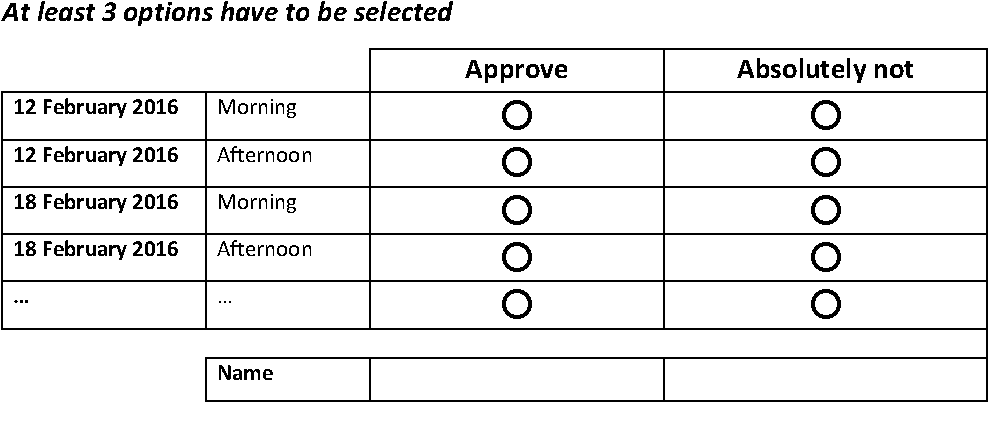
\includegraphics[width=.5\textwidth]{img/Voting.pdf}
\end{center}
%\end{parchment}

\begin{itemize}
\item Präferenzen von Studenten sollten nicht unterschiedlich hoch gewichtet werden
\item Lösung (Prüfplan) ist eine geteilte Entscheidung

\end{itemize}
\end{frame}

\begin{frame}[fragile]{Exam Scheduling: Core Model}
See \texttt{exam-scheduling-approval.mzn}:
\begin{lstlisting}
% Exam scheduling example with just a set of 
% approved dates and *impossible* ones
include "globals.mzn";
include "soft_constraints/soft_constraints.mzn";

int: n; set of int: STUDENT = 1..n; 
int: m; set of int: DATE = 1..m;
array[STUDENT] of set of DATE: possibles;
array[STUDENT] of set of DATE: impossibles;

% the actual decisions
array[STUDENT] of var DATE: scheduled;

int: minPerSlot = 0; int: maxPerSlot = 4;
constraint global_cardinality_low_up(scheduled % minPerSlot, maxPerSlot
constraint forall(s in STUDENT) (not (scheduled[s] in impossibles[s])); 
 
\end{lstlisting}
\end{frame}

\begin{frame}[fragile]{Exam Scheduling: Preferences}
See \texttt{exam-scheduling-approval.mzn}:
\begin{lstlisting}
% have a soft constraint for every student
nScs = n;
penalties = [ 1 | n in STUDENT]; % equally important in this case 

constraint forall(s in STUDENT) ( 
     (scheduled[s] in possibles[s]) <-> satisfied[s] ) ;
var DATE: scheduledDates;
% constrains that "scheduledDates" different 
% values (appointments) appear in "scheduled"
constraint  nvalue(scheduledDates, scheduled);

% search variants 
solve 
:: int_search(satisfied, input_order, indomain_max, complete)
search minimize_lex([scheduledDates, violateds]);   % pro teachers
%search minimize_lex([violateds, scheduledDates]); % pro students
\end{lstlisting}
\end{frame}


\begin{frame}[fragile]{Exam Scheduling: Realversuch}

\begin{itemize}
\item Gesammelte Präferenzen von 33 Studenten
\item verteilt über 12 mögliche Termine (6 Tage, Vormittag und Nachmittag)
\begin{itemize}
\item[-] \emph{Approval} set 
\item[-] \emph{Impossible} set 
\end{itemize}

\vspace*{2ex}

\item Kombiniert mittels \alert{Approval Voting} (schöne wahltheoretische Eigenschaften!)
\item Höchstens 4 pro Termin

\item Findet optimale Lösung sofort (61 msec) 
\begin{itemize}
\item[-] \emph{Jeder} Student stimmt Termin zu
\item[-] Wird mit der minimalen Anzahl von 9 Terminen erreicht
\end{itemize}
\item Eingesetzte Strategie:
\end{itemize}
\begin{lstlisting}
search minimize_lex([violateds, scheduledDates]); % pro students
\end{lstlisting}
\end{frame}

\begin{frame}{Take-away Messages}
\begin{parchment}[Take-away]
\centering 
\begin{enumerate}
\item Innovative Software steht vor \emph{Constraint-Optimierungsproblemen}
\vspace*{1ex}
\item Modellierung für leistungsfähige Algorithmik
\vspace*{1ex}
\item Algebraische Strukturen sind ``in'' \texttt{;-)}
\end{enumerate}
\end{parchment}

\url{schiendorfer@isse.de} \hfill Try it in your own projects!
\end{frame}